\subsection{Trigonometrische Funktionen}
\subsubsection{Die Winkelfunktionen rechtwinkliger Dreiecke}
Grundlegend gibt es drei Winkelfunktionen, welche auf rechtwinklige Dreiecke angewandt werden k"onnen:
\begin{itemize}
\item Sinus $\sin : \mathbb{R} \to \mathbb{R}, \mathbb{W} = \left[-1;1 \right]$
\item Kosinus $\cos : \mathbb{R} \to \mathbb{R}, \mathbb{W} = \left[ -1;1 \right]$
\item Tangens $\tan : \left( \mathbb{R} \setminus \left\{ k \pi + \frac{\pi}{2}, k \in \mathbb{Z} \right\} \right) \to \mathbb{R}, \mathbb{W} = \mathbb{R}$
\end{itemize}
\begin{warning}
	Der Tangens ist f"ur die Nullstellen des Kosinus nicht definiert denn
	\begin{equation*}
	\tan(x) := \frac{\sin(x)}{\cos(x)}
	\end{equation*}
\end{warning}
Die drei Seiten des Dreiecks werden als Hypotenuse (l"angste Seite des Dreiecks, -gegen"uber des rechten Winkels-), Ankathete (kurze Seite, welche am Winkel $\alpha$ anliegt), und Gegenkathete (Seite gegen"uber des Winkels $\alpha$) bezeichnet.
\begin{minipage}{0.45\textwidth}
\hfill
\begin{enumerate}
\item $\sin(\alpha)=\frac{\text{Gegekathete}}{\text{Hypotenuse}}$
\item $\cos(\alpha)=\frac{\text{Ankathete}}{\text{Hypotenuse}}$
\item $\tan(\alpha)=\frac{\sin(\alpha)}{\cos(\alpha)}= \frac{\text{Gegenkathete}}{\text{Ankathete}}$
\end{enumerate}
\end{minipage}
\begin{minipage}{0.45\textwidth}
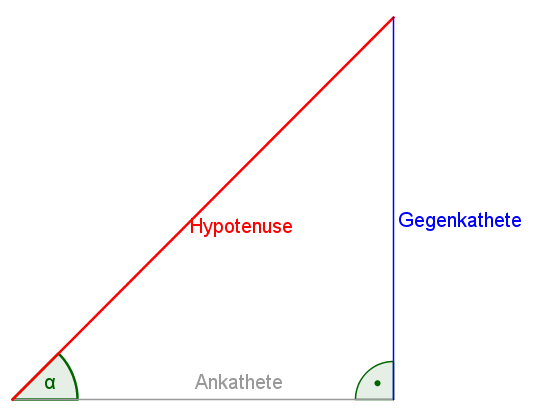
\includegraphics[width=1.0\textwidth]{pictures/TrigonDreieck}
\end{minipage}

\subsubsection{Der Einheitskreis}
Am besten sieht man die Eigenschaften der Winkelfunktionen bei der Betrachtung des \textcolor{red}{Einheitskreises}. Der Einheitskreis ist an sich nichts anderes als ein Kreis, mit Radius $r$ = 1 LE (L"angeneinheiten) und Kreismittelpunkt im Ursprung. Dabei ist die $x$-Koordinate des Punktes, am Ende der Hypotenuse des eingezeichneten Dreiecks, der Kosinuswert des Winkels Alpha und die $y$-Koordinate der Sinuswert. Der Tangens ist die Steigung der Hypotenuse. Der Zusammenhang zwischen Einheitskreis und den Funktionen ist in Abb. \ref{fig:circ} zu sehen.

\begin{figure}[h!]

\begin{tikzpicture}
% Axis
\draw[thick,-stealth,black] (-3,0)--(4,0) coordinate (A) node[below] {$x$}; % x axis
\draw[thick,-stealth,black] (0,-3)--(0,3) node[left] {$y$}; % y axis
\draw[black,thin] (0,0) circle (2.5cm);
\node[black,below] at (2.7,0) {1};
\node[black,above] at (0.2,-3.2) {1};

\draw[ultra thick,orange] (0,0) -- (\theangle:2.5cm |- 0,0) node[midway,above] {$\cos(\alpha)$}; % UpOn y axis

\draw (1,0) arc (0:\theangle:1) node at ($(\theangle/2:0.7)$) {$\alpha$};
\draw[dashed, cyan] (\theangle:2.5cm) -- (\theangle:2.5cm |- 0,0) node[sloped, rotate=180, yshift=8pt, midway] {$\sin(\alpha)$}; % vertical line
\draw[ultra thick,red,rotate=\theangle] (0,0) -- (2.5,0) coordinate (B); 

\draw[dashed,red] (0,0) -- (-2.5,-2.097);

\draw[ultra thick, blue] (-2.5,0) -- (-2.5,-2.097) node[sloped, midway,below] {$\tan(\alpha)$};;

\foreach \x in {0,30,...,360} {\filldraw[black] (\x:2.5cm) circle(1pt);};
\foreach \x/\xtext in {
        30/\frac{\pi}{6},
        60/\frac{\pi}{3},
        120/\frac{2\pi}{3},
        150/\frac{5\pi}{6},
        210/\frac{7\pi}{6},
        240/\frac{4\pi}{3},
        300/\frac{5\pi}{3},
        330/\frac{11\pi}{6}
        }
    \draw (\x:2.8cm) node {\tiny $\xtext$};
 \foreach \x/\xtext in {
        90/\frac{\pi}{2}}
        \draw (\x:2.7cm) node[xshift=4pt] {\tiny $\xtext$};    
 \foreach \x/\xtext in {
        270/\frac{3\pi}{2}}
        \draw (\x:2.7cm) node[xshift=-5pt] {\tiny $\xtext$};  
 \foreach \x/\xtext in {
        180/\pi,
        360/2\pi}
        \draw (\x:2.7cm) node[yshift=4pt] {\tiny $\xtext$};             

\begin{scope}
\begin{axis}[
    thick,
    y=2.5cm,
    axis lines=center,
    xmin=0, xmax=360,
    ymin=-1, ymax=1,
    anchor=origin, at=(A),
    xshift=3ex,
    enlarge y limits,
    enlarge x limits=upper,
    samples=90,
    xtick={0,30,...,360},
xticklabels={0,
    $\frac{\pi}{6}$,
    $\frac{\pi}{3}$,
    $\frac{\pi}{2}$,        
    $\frac{2\pi}{3}$,
    $\frac{5\pi}{6}$,
    $\pi$,
    $\frac{7\pi}{6}$,
    $\frac{4\pi}{3}$,
    $\frac{3\pi}{2}$,        
    $\frac{5\pi}{3}$,
    $\frac{11\pi}{6}$,
    $2\pi$
    },
    tick label style={font=\tiny},
    ]
    \addplot[domain=0:\theangle,ultra thick, no markers,cyan] {sin(x)} coordinate (C);
    \addplot[domain=\theangle-1:\theangle,ultra thick, no markers,cyan] {sin(x)-sin(x)} coordinate (K);

\end{axis}
\draw [dashed,red, thick] (B) -- (C);
\draw [dashed,cyan, thick] (C) -- (K);
\end{scope}
\tkzDrawPoints(B);
\end{tikzpicture}
\caption{Einheitskreis (links) und die Sinusfunktion (rechts).}
\label{fig:circ}
\end{figure}

\subsubsection{Winkelma"s und Bogenma"s}
Bisher haben wir immer mit Winkelma"sen gerechnet, wie zum Beispiel $\alpha = 45^\circ$. Neben dieser M"oglichkeit, Winkel auszudr"ucken, gibt es auch noch das Bogenma"s $b = 2\pi \ rad$. Das Bogenma"s ist die L"ange des Kreisbogens mit dem Radius $r = 1$ unter einem bestimmten Winkel. Die Umrechnung ist einfach
\begin{equation*}
rad(\alpha) = 2\pi \frac{\alpha}{360} rad \text{ f"ur } \alpha \in \left[ 0^\circ;360^\circ \right] \quad rad^{-1}(b) = 360 \cdot {\frac{b}{2\pi}}^\circ \text{ f"ur } b \in \left[0;2\pi\right]
\end{equation*}
Wie ein Winkelwert mit $^\circ$ gekennzeichnet wird, so kennzeichnet man das Bogenma"s mit dem W"ortchen "'$rad$"'.
\begin{warning}
	An den meisten "'h"oheren"' Schulen wird das Bogenma"s bevorzugt.\\
	Ihr solltet eure Taschenrechner dementsprechend umstellen (meist ist dies "uber eine \textit{Mode}-Taste zu bewerkstelligen)
\end{warning}

\begin{figure}[h!]
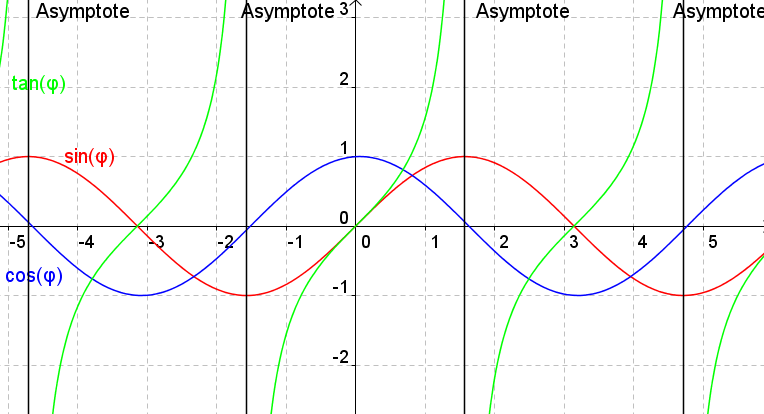
\includegraphics[width = 13 cm, height = 5 cm]{pictures/Winkelfunktionen}
\caption{Funktionsgraphen von Sinus, Kosinus und Tangens}
\end{figure}

\subsubsection{Nullstellen, Asymptoten und Symmetrie}
Alle Winkelfunktionen sind periodisch. Deshalb treten auch ihre Nullstellen in gleichbleibenden Abst"anden auf.
\begin{itemize}
\item Sinusfunktion:
\begin{equation*}
 \sin(x) = 0 \iff x \in \left\{ k \pi, k \in \mathbb{Z} \right\},
\end{equation*}
was sich mit den Nullstellen des Tangens deckt.
\item Kosinusfunktion: 
\begin{equation*}
 \cos(x) = 0 \iff x \in \left\{ k \pi + \frac{\pi}{2}, k \in \mathbb{Z} \right\},
\end{equation*}
was sich mit den Definitionsl"ucken des Tangens deckt.
\end{itemize}
Des Weiteren besitzt die Tangensfunktion eine periodisch auftretende senkrechte Asymptote an den Nullstellen des Kosinus.
Betrachtet man die Graphen im Hinblick auf ihre Symmetrie bez"uglich des Koordinatensystems, stellt man fest, dass die Sinus- und Tangesnsfunktion \textbf{punktsymmetrisch} zum Ursprung (ungerade) und die Kosinusfunktion achsensymmetriesch zur $y$-Achse (gerade) ist.

\subsubsection{Periodizit"at}
Eine Funktion ist dann \textcolor{red}{periodisch}, wenn es eine Konstante p gibt, f"ur die gilt:
\begin{equation*}
f(x+p) = f(x), \forall x\in\mathbb{D}
\end{equation*}
Diese Definition sagt eigentlich nichts anderes aus, als dass sich die Funktion st"andig im gleichen Abstand wiederholt.
